%The document is report. 
\documentclass[12pt]{report}

%Allows custom headers. 
\usepackage{fancyhdr}
%Allows two columns; used for title page. 
\usepackage{multicol}
%Sets margin and spaces header inside of margin.
\usepackage[margin=1in,headheight=15pt]{geometry}
%Allows use of images.
\usepackage{graphicx}
%used for labeling of the lists.
\usepackage{scrextend}
\addtokomafont{labelinglabel}{\sffamily}
%Used for better customization of table cells. 
\usepackage{makecell}
%For listing and formatting code.
\usepackage{listings}
\usepackage{color}
%used for the product requirements list.
\usepackage[ampersand]{easylist}
%Package to allow cleanly changing the headers. 
\usepackage{titlesec}
%Removes exesive default chapter numbering.
\titleformat{\chapter}[display]{\normalfont\huge\bfseries}{}{0pt}{\Huge}
%By default, there's extra margins at the top of chapter pages. 
\titlespacing*{\chapter} {0pt}{-40pt}{10pt}
%Remove horizontal fancy header line.
\renewcommand{\headrulewidth}{0pt}
%Adds our custom text to the left header.
\lhead{JP: To The Rescue!}
%Removes the default text from the right header.
\rhead{}

%Allows clickable PDF Hyperlinks.
\usepackage[linktocpage=true]{hyperref}
\hypersetup{colorlinks=true,linkcolor=blue,anchorcolor=blue,citecolor=blue,filecolor=blue,urlcolor=blue,bookmarksnumbered=true}
%Removes the default red borders for the hyperlinks.
\hypersetup{pdfborder = {0 0 0}}
\usepackage[all]{hypcap}

%Begins the layout of the document. 
\begin{document}
	
\title{JP Project To the Rescue!}
\author{Robert Mooers}
%\maketitle

%Custom layout titlepage.
\begin{titlepage}
	%Centering all text within the column.
	\centering
	%Title of the report.
	{\huge\bfseries
		Junior Project Proposal \par}
	%A short space between the title and the author.
	{\huge\bfseries
		To The Rescue! \par}
	
	%Moving down half the page. 
	\vfill
	
	%Adding the custom image.
	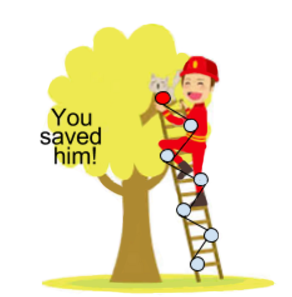
\includegraphics{Tree}
	
	\vspace{2cm}
	\begin{multicols}{2}
		{\Large\bfseries
			Submitted By: \par}
		%A short space between the title and the author.
		\columnbreak
		\begin{flushleft}
		{	
			\Large\itshape Lake Sain-Thomason \\
			\ \ \normalsize\normalfont \href{mailto:lakesainthomason@gmail.com}{lakesainthomason@gmail.com} \\
			\Large\itshape Matthew Del Fante \\
			\ \ \normalsize\normalfont \href{mailto:matthewdelfante@gmail.com}{matthewdelfante@gmail.com} \\
			\Large\itshape Robert Mooers \\
			\ \ \normalsize\normalfont \href{mailto:Robert.Mooers@oit.edu}{robert.mooers@oit.edu} \\
			\Large\itshape Stephanie Vetter-Derosier \\
			\ \ \normalsize\normalfont \href{mailto: Stephanie.Vetter@oit.edu}{ Stephanie.Vetter@oit.edu}
		\par}
		\end{flushleft}
	\end{multicols}
	
	\begin{multicols}{2}
		{\Large\bfseries
			Submitted To: \par}
		%A short space between the title and the author.
		\columnbreak
		\begin{flushleft}
			{\Large\itshape Todd Breedlove \\
				\ \ \normalsize\normalfont \href{mailto:Todd.Breedlove@oit.edu}{Todd.Breedlove@oit.edu} \\
			\par}
		\end{flushleft}
	\end{multicols}
	
	%Moving down half the page. 
	\vfill
	
	%The date, generated.
	{\large \today \par}
	%The class written for.
	{\large V1.1 \par}
	%Manually moving to next column.
	\footnotesize
	%Displaying uninterpreted text. 

%Ending the title page. 
\end{titlepage}


%Frontmater in lower case roman numerals.
\pagenumbering{roman} 

%Legal Notice, Copyright Notice Page

	%Adds page number and header to pages that default to not having it.
	\thispagestyle{fancy}
	\subsection*{Legal Notice}
	\phantomsection
	\addcontentsline{toc}{chapter}{Legal Notice}\label{subsec:LegalNotice}
		\paragraph{}\ \ ‘To the Rescue!’ makes no warranties of representation of any kind concerning the accuracy or suitability of the information contained in this document for any purpose. All such information is provided “as is” and with specific disclaimer of any warranties of merchantability, fitness for purpose, title and/or non-infringement. In no event shall To The Rescue!, its employees or agents be liable for any direct, indirect or consequential damages resulting from the information provided in this document. This exclusion and limitation only applies to the contrary in any written license or subscription agreement from ‘To the Rescue!’ in respect of this document or references. 
		
	\vfill
	 
	\subsection*{Copyright Notice}
	\phantomsection
	\addcontentsline{toc}{chapter}{Copyright Notice}\label{subsec:CopyrightNotice}
		{\bfseries Copyright ©2016-2017 ‘To the Rescue!’. All Rights Reserved}
		\paragraph{}\ \ The copyright on all materials provided in this document is held by ‘To the Rescue!’ or by the original creator of the material. Except as stated herein, none of the material may be copied, reproduced, distributed, republished, translated, displayed, posted, communicated to the public by telecommunication or transmitted in any form of by any means, including, but not limited to, electronic, mechanical, photocopying, recording, or otherwise, without the prior written permission of the copyright holder. Permission is granted to display, copy and distribute the materials in this document for personal, noncommercial use provided no modifications are made to the materials and all copyright and other proprietary notices contained in the materials are retained. This permission terminates automatically if you breach any of these terms or conditions. Upon termination, any printed materials must be immediately destroyed. Any unauthorized use of any material contained in this document may violate copyright laws, trademark laws, the laws of privacy and publicity, and communications regulations and statutes. All rights, titles and interest not expressly granted are reserved.    
	\pagebreak
	\subsection*{Revision History}
	\phantomsection
	\addcontentsline{toc}{chapter}{Revision History}\label{subsec:RevisionHistory}
	\begin{tabular}{| l | l | l | l | l |}
		\hline		
		\bfseries Authors & \bfseries Date & \bfseries Version &\bfseries File Name & \bfseries Comments \\ \hline
		\normalfont \makecell[l]{Lake Sain-Thomason,\\ Matthew Del Fante,\\ Robert Mooers,\\ Stephanie Vetter-Derosier} & \makecell[l]{October 16,\\ 2016} & v1.0 & Proposal.pdf &\makecell[l]{Formatted brainstormed \\ content into a cohesive \\ document.	} \\ 
		
		\hline
			
		\normalfont \makecell[l]{Lake Sain-Thomason,\\ Matthew Del Fante,\\ Robert Mooers,\\ Stephanie Vetter-Derosier} & \makecell[l]{October 20,\\ 2016} & v1.1 & Proposal1-1.pdf &\makecell[l]{Modified Database \\ information in \\  section 4.1.	} \\ \hline	
	\end{tabular}
%Signature Page	
	\pagebreak
	\subsection*{Signature Page}
	\phantomsection
	\addcontentsline{toc}{chapter}{Signature Page}\label{subsec:SignaturePage}
	\vspace{1cm}
	\noindent
	This document accepted by:
	
	\vspace{2cm}
	
	\begin{minipage}[t]{.5\textwidth}
		\begin{tabular}{c}
			\hline		
			\makecell[{{p{8cm}}}]{\centering Signature (Todd Breedlove)}
		\end{tabular}
	\end{minipage}
	\begin{minipage}[t]{.5\textwidth}
		\centering
		\begin{tabular}{c}
			\hline		
			\makecell[{{p{3cm}}}]{\centering Date}
		\end{tabular}
	\end{minipage}
	
	\vfill
	
	\noindent
	This document submitted by:
	
	\vspace{2cm}
	\begin{minipage}[t]{.5\textwidth}
		\begin{tabular}{c}
			\hline		
			\makecell[{{p{8cm}}}]{\centering Signature (Lake Sain-Thomason)}
		\end{tabular}
	\end{minipage}
	\begin{minipage}[t]{.5\textwidth}
		\centering
		\begin{tabular}{c}
			\hline		
			\makecell[{{p{3cm}}}]{\centering Date}
		\end{tabular}
	\end{minipage}
	
	\vspace{2cm}
	
	\begin{minipage}[t]{.5\textwidth}
		\begin{tabular}{c}
			\hline		
			\makecell[{{p{8cm}}}]{\centering Signature (Matthew Del Fante)}
		\end{tabular}
	\end{minipage}
	\begin{minipage}[t]{.5\textwidth}
		\centering
		\begin{tabular}{c}
			\hline		
			\makecell[{{p{3cm}}}]{\centering Date}
		\end{tabular}
	\end{minipage}
	
	\vspace{2cm}
	
	\begin{minipage}[t]{.5\textwidth}
		\begin{tabular}{c}
			\hline		
			\makecell[{{p{8cm}}}]{\centering Signature (Robert Mooers)}
		\end{tabular}
	\end{minipage}
	\begin{minipage}[t]{.5\textwidth}
		\centering
		\begin{tabular}{c}
			\hline		
			\makecell[{{p{3cm}}}]{\centering Date}
		\end{tabular}
	\end{minipage}
	
	\vspace{2cm}
	
	\begin{minipage}[t]{.5\textwidth}
		\begin{tabular}{c}
			\hline		
			\makecell[{{p{8cm}}}]{\centering Signature (Stephanie Vetter-Derosier)}
		\end{tabular}
	\end{minipage}
	\begin{minipage}[t]{.5\textwidth}
		\centering
		\begin{tabular}{c}
			\hline		
			\makecell[{{p{3cm}}}]{\centering Date}
		\end{tabular}
	\end{minipage}
	

%The generated table of contents. 
\tableofcontents
	\thispagestyle{fancy}
\addcontentsline{toc}{chapter}{Table of Contents}
%Forces table of contents to have its own page.
\newpage

%Use fancy headers for non-specific pages. 
\pagestyle{fancy}
%Change page numbers to arabic numerals. 
\pagenumbering{arabic}

\chapter{Introduction}
	\label{ch:intro}
	\thispagestyle{fancy}
	
	\section{Purpose}
	\label{sec:Purpose}
	\paragraph{}\ \ The purpose of this document is to propose the design and implementation of ‘To the Rescue!’. The sections and subsections following are dedicated to define or describe the format of this document or the intended design plans. If this proposal is accepted, it will serve as a guide to constrain the implementation process.  
	
	\section{Scope}
	\label{sec:Scope}
	\paragraph{}\ \ The scope of this document is limited to project management, general system discussion, and a description of the product requirements which will describe in limited detail the intended design features and functionality. Also included is the specific functionality of modules and otherwise discrete functionalities that may later be added to the system.
	\section{Intended Audience}
	\label{sec:IntendedAudience}
	\paragraph{}\ \ The audience this document is intended for includes Todd Breedlove, all members of ‘To the Rescue!’, and any third party interested or curious about this project.
	
\chapter{Project Management}
\thispagestyle{fancy}

	\section{Change Management Procedures}
	\paragraph{}\ \ In the event there is a change request to modify the system, the CAT Team will be informed about the change. The Change Request Form can be found in Appendix B and will provide the information outlined in Section 2.2 of this document. 
	
	\section{CAT Team, Timelines, and Documentation}
	\begin{labeling}{Impact Analysis}
		\item [CAT Team] The CAT Team will consist of the members of ‘To the Rescue!’ and Todd Breedlove. The team will evaluate the impact a change will have on the developing system. Submitted changes can be accepted or rejected by the team with a brief statement explaining the reasons for the decision. Submitted changes – whether accepted or rejected – will be archived in a cloud storage medium managed by the members of ‘To the Rescue!’.
		\item [Medium] Any changes must be submitted, in the format presented by the Change Request Form (Appendix B), by any member of the CAT Team. Submission is to be physical copy only – digital submissions will not be accepted. A form for each CAT Team member must be submitted for the change request to be considered.
		\item [Response Time] The Change Request Form will be processed over the course of two to three business days. Responses will be emailed to the addresses detailed on the submitted Change Request Form. 
		\item [Impact Analysis] Before a change moves forward, the impact that it will have on the system’s development timeline must be inspected. If a change is proposed that would move the final production version of the system past the maximum allotted time, the change will be automatically denied. 
		\item [Time Frame] In the event that a change is accepted, the development timeline of the system will be modified to accommodate the change. This modification is allowed to decrease or increase the development timeframe.  
	\end{labeling}
	\section{Software Delivery, Installation, and Acceptance Criteria}
		\paragraph{}\ \ Software delivery will be distributed to all interested parties for evaluation by the end of spring term of the 2016 -- 2017 school year. Included in the delivery will be a web application, written documentation of system requirements and written documentation for the startup process. Acceptance criteria will be based on completeness and operability of the provided items and software. 
	\section{Documentation and Online Help}
		\paragraph{}\ \ Software documentation will be provided in written format. Documentation provided will detail the system requirements, startup process, and operation of the software described by this document. 
	\section{Project Risks}
		\paragraph{}\ \ Risks for this project involve the developers learning the proposed front end programming language (JavaScript) and the environment that the proposed application will run (Google Chrome). Also, the application does not have a defined amount of content required, leaving the application feeling incomplete if the developers do not fill it properly.
	\section{Customer Responsibilities}
		\paragraph{}\ \ The customer will be responsible for providing their own mobile device or personal computer loaded with Google Chrome.
	\section{Status Reporting}
		\paragraph{}\ \ Status reporting will be submitted weekly in memo format to Todd Breedlove. The report will include the following:
		
		\begin{itemize}
			\item Work completed during the current week
			\item Work to be completed during the next week
			\item Issues found during current week’s work
		\end{itemize}
		
\chapter{System General Description}
\thispagestyle{fancy}
	\section{Problem Statement}
		\paragraph{}\ \ We will be writing a children's learning application as a progressive web application. The application will consist of numerous mini games that will align with the Oregon State Standards for Kindergarten.
		
		\paragraph{}\ \ The main interface will be a game map consisting of mini games along a path. The goal is to complete all mini games and rescue an animal at the end of the path. Once the user rescues an animal, the animal will be added to his or her “Animal Sanctuary”. The Animal Sanctuary represents the progress and achievements made by the user. The user will move to the next map after rescuing the animal. The difficulty of the mini games will increase, decrease, or remain the same depending on the user's mini game progress/success. A congratulatory splash screen will appear once all the maps have been completed. The user may play through the game as many times as he or she may like to continue to add animals to the sanctuary.
				
		\paragraph{}\ \ Upon launching the application, the user will have the option to create a user account, login to an existing account, or play the game without a user account. A user account will allow the user to create profiles and pick avatars to associate with these profiles. The user account tracks and saves the user's progress throughout the game. The user's animal collection will also be saved. In free play mode, the user's progress and animal collection are not saved. 
		
		\paragraph{}\ \ Users will not be required to login to the app before they can use it, but a login will be required to create multiple profiles and to move saves between different devices. The user will be able to create an account from within the application with only an email, which will be his or her username, and a password. Passwords will be encrypted before being sent from the client to the server.
		
		\paragraph{}\ \ Upon logging in or creating a new account, the choose profile page will appear. From this page, the user will be able to choose to continue an existing profile or to create a new profile.
				
		\paragraph{}\ \ The main menu will appear once the user selects a profile, or if they choose to play without an account. From the main menu, the user may choose “Play”, which takes them to the game map, or the user may select “Options” to customize game play. In the options menu, the user may toggle sound, set the difficulty level of the mini games, and filter mini games by subject.
				
		\paragraph{}\ \ User information that will be stored in the database includes the user's email (username), password, profile name, profile avatar, game progress and the animals collected. References to the game map images will be stored in the database as well. Mini game information including a reference to the game code, game data and statistics for the games will be located in the database. Lastly, the database will have the game's state stored in it as well.
		
	\section{Perspective}
	
		\subsection{History}
			\paragraph{}\ \ The idea for ‘To the Rescue!’ was a collaborative group effort that supports the abilities and interests of all group members. The ‘To the Rescue!’ project also provides opportunities for all members of the team to learn by experiencing new design and programming challenges. This project requires creativity and diversity to keep the content new and engaging. The developers wanted a project that would incorporate the interests of all members. This project also promotes education and can be extended to reach users of different ages and learning levels. 
		\subsection{Background}
			\paragraph{}\ \ Matthew Del Fante started programming two years ago and is proficient with the object-oriented and imperative programming paradigms. Programming languages that Matt is knowledgeable on include C++, C, C\#, JavaScript and QML.
			
			\paragraph{}\ \ Stephanie Vetter-Derosier has a background in early childhood and elementary education. She has been programming for two years and has experience in C++, C, C\#, Java, and QML. Stephanie had the opportunity to intern at a data analysis company in 2016. During her internship, she gained experience in project planning and development, Java, and automated software testing.
			
			\paragraph{}\ \ Lake Sain-Thomason is a fourth year software engineering student. After his sophomore year at SOU, he transferred to OIT to pursue a higher education. He is familiar with many languages such as C\#, C++, Java, C, and Obj-C. 
			
			\paragraph{}\ \ Robert Mooers has three years of programming experience, having primarily used C, C++, C\#, Java, Python, and QML. Robert is also proficient in graphics design, with experience in photo editing and vector graphics.
			
		\subsection{Prior Release}
			\paragraph{}\ \ There have been no prior releases at the time this document was written.
	\section{Major Subsystems}
		\paragraph{}\ \ This application is comprised of three major subsystems, the progressive web app client, the server, and the database. The progressive web app client will contain the user interface, and interact with the user. Individual games will be played within the client, and the results and statistical data will be sent to the server. The server will accept messages from clients including state, and will respond with the next action required for the client. The database will be used to hold user data and game information.
			
	\section{Relation of System to Existing System(s)}
		\paragraph{}\ \ ‘To the Rescue!’ will use libraries packaged with the ASP.NET Model View Controller framework. We intend on using open source/free images, Windows Voice Recorder for audio and open source/free audio clips.
	\section{Hardware Platform Description}
		\paragraph{}\ \ Minimum Hardware Requirements for Google Chrome, the supported browser of ‘To the Rescue!’, is: Windows 7, Windows 8, Windows 10 or later and an Intel Pentium 4 processor or later that is SSE2 capable. Required internet speed for ‘To the Rescue!’ is 4Mbps or higher.
	\section{Software Platform Description}
		\paragraph{}\ \ ‘To the Rescue!’ will be tested and intended for the Google Chrome web browser, but should be able to run on any web browser.
\chapter{Product Requirements}
\thispagestyle{fancy}
	\section{Functional}
		\ListProperties(Progressive*=3ex)
		\begin{easylist}
			& Navigate to web application 
			&& Supported on Google Chrome
			&& Supported on mobile devices
			&&& Progressive web application
			&& Display Initial Splash Screen for Parents
			&&& Button to Login
			&&&& Display drop down login box
			&&& Button to Create Account
			&&&& Display Create Account drop down box
			&&& Button to play without an Account or saving progress
			&&&& No login or account required
			&&&& Avatar chosen for user
			&&&& User unable to enter name for avatar
			&&&& User progress is not saved
			&&&& Mini-games start at easiest difficulty level
			&& Background music
			& Login-Drop Down Box
			&& Option for user to login to existing account
			&&& User enters username (email) and password
			&&&& Go to Choose Profile
			&&& Button to reset password
			&&&& Send a temporary password to email
			&&&& User enters temporary password
			&&&& Prompted to enter new password
			& Choose Profile Page
			&& List all profiles for the account
			&& User selects a profile 
			&&& Go to Main Menu
			&& Button to Create new profile
			&&& Go to Create New Profile page
			&& Drop down box to delete a profile
			&&& Prompt user to enter profile name and account password to delete profile
			& Create New Account-Drop Down Box
			&& User enters email address for username
			&&& Check that username aren't already in database 
			&& User creates a password
			&&& Alpha characters and numerics only
			&& Redirect to Choose Profile Page
			& New Profile page
			&& User enters profile name 
			&& User selects an avatar for profile pic and game character
			&&& Display all available avatars
			&& After creating the profile, redirect to Choose Profile Page
			& User accounts
			&& Account information stored in database
			&&& Profile name
			&&& Profile avatar
			&&& Email login (username)
			&&& Login password
			&&&& Encrypt before transmitting to server
			&&& User game progress
			&&&& Map level
			&&&& Last mini-game completed (location on path)
			&&&& Performance statistic (success percentage)
			&&&&& Implicitly determines mini-game difficulty
			&&&& Animal collection
			& Main Menu
			&& Main menu appears once the user has picked a profile or is playing in free play mode
			&&& Main menu background music
			&& User may choose to go to Animal Sanctuary
			&&& Display animals that user has rescued
			&&& Animals make noise and small movement when clicked
			&&& Animals move around Sanctuary
			&&& Button to go back to Main Menu
			&&& Fun Facts listable for animals
			&&& Background music
			&& User may choose to go to Options Menu
			&&& Options menu requires password entry to change anything
			&&& Button to Log Out
			&&&& Automatically default to staying logged in when the app closed
			&&& User may toggle sound
			&&& User may filter mini-games by subject
			&&&& Play only literacy games
			&&&& Play only mathematics games
			&&&& Play a mix of literacy and mathematics games
			&&&& Content based on Oregon State Standards/Common Core Standards (CCS) for Kindergarten
			&&& User may choose to set game difficulty
			&&&& Defaults to easiest difficulty
			&&&& Button to switch/create/delete profile
			&&&& Go to Choose Profile Page
			&&& Button to go back to Main Menu
			&& User may choose to play the game
			&&& Restore user’s progress and mini-game difficulty if logged into an existing account
			& Game Play:Maps and Mini-Games
			&& Display game play Map
			&&& Map contains a path with nodes as mini-game stopping points
			&&& User’s avatar is shown on map at current location
			&&& User stops at each node along the path
			&& Sidebar Options Menu
			&&& Button to exit map and return to Main Menu
			&&& Button to go to Options
			&&& Button to go to Animal Sanctuary 
			&& Must play mini-game at current node to move to next node
			&&& Must play entire mini-game to “pass”
			&&&& User does not pass or fail based on performance
			&&&& User praised for excellent work regardless of performance
			&&&& Mini-games reinforce correct answers and positively correct wrong answers
			&&&& Save user’s progress and performance statistic in database after each completed mini-game
			&&& Mini-games are randomly selected for maps
			&&&& Mini-games appear more than once
			&&&&& Different content when they do appear multiple times
			&&&& Track mini-game appearance so same game doesn’t appear multiple times in a row
			&&&& Mini-game content is randomly selected from database
			&& At end of the map is an animal to rescue
			&&& User rescues animal after completing all mini-games on map
			&&& The rescued animal is moved to user’s Animal Sanctuary
			&& Once a map is completed, user moves to the next map
			&&& Algorithm to determine if mini-game difficulty should increase, decrease, or remain the same based on user’s ability to complete mini-games on previous map
			&& Display a congratulatory splash screen when all maps are completed
			&&& Return to Main Menu
			&&&& User may play game again from beginning
			&&&& Animals are preserved in the Sanctuary
			& Database
			&& Create table for user accounts
			&&& Email(username)
			&&& Encrypt Password
			&& Create table for user profiles
			&&& Reference to account
			&&& Profile Name
			&&& Avatar ID
			&& Create table of animal collections (for each profile)
			&&& Animal ID
			&&& Profile ID
			&& Create tables for image references
			&&& Available avatars
			&&& Game maps
			&&& Animals to rescue
			&& Create table for mini-game content(data)
			&&& Reference to the location of the mini game code
			&&& General game data such as:
			&&&& Colors, words and reference to images
			&&&& Math sequences 
			&&&& Sight words and letters
			&&&& Numbers and corresponding words
			&& Create user progress table (stores upon mini-game completion)
			&&& Stores current map
			&&& Stores location (node) on map
			&&& Stores the ID of the last three mini-games completed
		\end{easylist}
		
	\newpage
	\section{Performance}
		\paragraph{}\ \ ‘To the Rescue!’ will run at 60 frames per second to provide smooth transitions between pages and silky movements of small characters. Older devices may experience a lower or choppy framerate that do not fit the hardware specifications. 
	
	\section{Reliability}
		\paragraph{}\ \ ‘To the Rescue’ will try to maintain 95\% reliability for up to 30 concurrent users. It is important that users are able to rely on the application functioning properly, but the server may unexpectedly go down. Thus, 95\% reliability is reasonable. If more than 30 users use the application concurrently, the application will become less reliable.
	\section{Data Description}
		\paragraph{}\ \ ‘To the Rescue!’ will be serving web pages, including images, audio, and JavaScript. Data will be transferred from the database and to the database through an internet connection. The transfer rate will be 4 Mbps with a maximum page load time of 2 seconds.
	\section{Security and Safety}
		\paragraph{}\ \ All passwords will be encrypted before being sent off to the database, and users are logged out when the application is closed. 
	\section{Constraints}
		\paragraph{}\ \ 'To The Rescue!' content will be based on the Oregon State Common Core Standards for Kindergarten.
\chapter{User Profiles}	
	\paragraph{}\ \ The users of this software will be parents who create accounts for their children and the children use the application. The target users are children at a preschool and kindergarten learning level.
	
\newpage
\appendix
\chapter{A - Glossary of Terms} 
\small
\label{App:AppendixA}
\thispagestyle{fancy}	
	
	\begin{labeling}{Progressive Web App}
		\item [Progressive Web App] A new way to create web applications that is responsive to a user's mobile device. Progressive Web Apps allows users to add the app to the home screen of the user's mobile device with one click, and does not require installation. 
	\end{labeling}
	
	
\newpage
\appendix
\chapter{B - Change Request Form} 
\small
\label{App:AppendixB}
\thispagestyle{fancy}	
	
	\vspace{2cm}
	\begin{minipage}[t]{.33\textwidth}
		\centering
		\begin{tabular}{c}
			\hline		
			\makecell[{{p{4cm}}}]{\centering Name (Print)}
		\end{tabular}
	\end{minipage}
	\begin{minipage}[t]{.33\textwidth}
		\centering
		\begin{tabular}{c}
			\hline		
			\makecell[{{p{4cm}}}]{\centering Email Address}
		\end{tabular}
	\end{minipage}
	\begin{minipage}[t]{.33\textwidth}
		\centering
		\begin{tabular}{c}
			\hline		
			\makecell[{{p{3cm}}}]{\centering Date}
		\end{tabular}
	\end{minipage}
	
	\vspace{2cm}
	\noindent
	Change Request:
	
	\vfill
	\noindent
	Purpose for Change Request:
	
	\vfill
	\noindent
	Additional Comments:
	\vfill	
	
	
\end{document}          
